% !TEX TS-program = pdflatex
% !TEX encoding = UTF-8 Unicode

% This is a simple template for a LaTeX document using the "article" class.
% See "book", "report", "letter" for other types of document.

\documentclass[11pt]{article} % use larger type; default would be 10pt

\usepackage[utf8]{inputenc} % set input encoding (not needed with XeLaTeX)

%%% Examples of Article customizations
% These packages are optional, depending whether you want the features they provide.
% See the LaTeX Companion or other references for full information.

%%% PAGE DIMENSIONS
\usepackage{geometry} % to change the page dimensions
\geometry{a4paper} % or letterpaper (US) or a5paper or....
% \geometry{margin=2in} % for example, change the margins to 2 inches all round
% \geometry{landscape} % set up the page for landscape
%   read geometry.pdf for detailed page layout information

\usepackage{graphicx} % support the \includegraphics command and options

% \usepackage[parfill]{parskip} % Activate to begin paragraphs with an empty line rather than an indent

%%% PACKAGES
\usepackage{booktabs} % for much better looking tables
\usepackage{array} % for better arrays (eg matrices) in maths
\usepackage{paralist} % very flexible & customisable lists (eg. enumerate/itemize, etc.)
\usepackage{verbatim} % adds environment for commenting out blocks of text & for better verbatim
\usepackage{subfig} % make it possible to include more than one captioned figure/table in a single float
% These packages are all incorporated in the memoir class to one degree or another...

%%% HEADERS & FOOTERS
\usepackage{fancyhdr} % This should be set AFTER setting up the page geometry
\pagestyle{fancy} % options: empty , plain , fancy
\renewcommand{\headrulewidth}{0pt} % customise the layout...
\lhead{}\chead{}\rhead{}
\lfoot{}\cfoot{\thepage}\rfoot{}

%%% SECTION TITLE APPEARANCE
\usepackage{sectsty}
\allsectionsfont{\sffamily\mdseries\upshape} % (See the fntguide.pdf for font help)
% (This matches ConTeXt defaults)

%%% ToC (table of contents) APPEARANCE
\usepackage[nottoc,notlof,notlot]{tocbibind} % Put the bibliography in the ToC
\usepackage[titles,subfigure]{tocloft} % Alter the style of the Table of Contents
\renewcommand{\cftsecfont}{\rmfamily\mdseries\upshape}
\renewcommand{\cftsecpagefont}{\rmfamily\mdseries\upshape} % No bold!

\setlength{\parindent}{0pt}
%%% END Article customizations

%%% The "real" document content comes below...

\title{Visualisierung mittels Vampir}
\author{Merlin Steuer, Merlin Koglin, Timon Vosberg}
\date{} % Activate to display a given date or no date (if empty),
         % otherwise the current date is printed 

\begin{document}
\maketitle
\section{Vampir}
Wir haben für unsere Visualisierung die Implementierung mit den blockierenden MPI Routinen verwendet, da die nicht-blockierende Version kein übersichtliches Bild ergeben haben.
Das verwendete Jobscript:
\begin{verbatim}
#SBATCH -N 1 -n 12
#SBATCH --output=circle.out

mpiexec ./circle-blockierend 30
\end{verbatim}
Also 12 Prozesse auf einem Knoten mit der Länge 30.

Nach dem Starten von Vampir, fällt als erstes auf, das \verb|MPI_Init| die meiste Zeit in Anspruch genommen hat und man in der Timeline sehr weit reinzoomen muss,
um die anderen Vorgängen zu sehen:\\
~\\
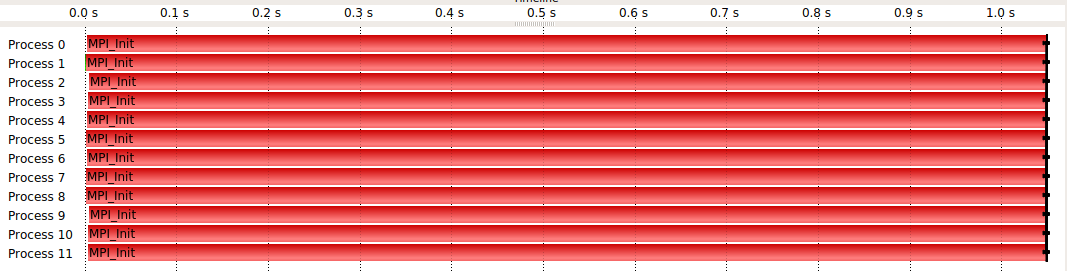
\includegraphics[width=1\textwidth]{./vampir/start.png}

\newpage
Hier ein Bild mit Zoom im Millisekunden Bereich:\\
~\\
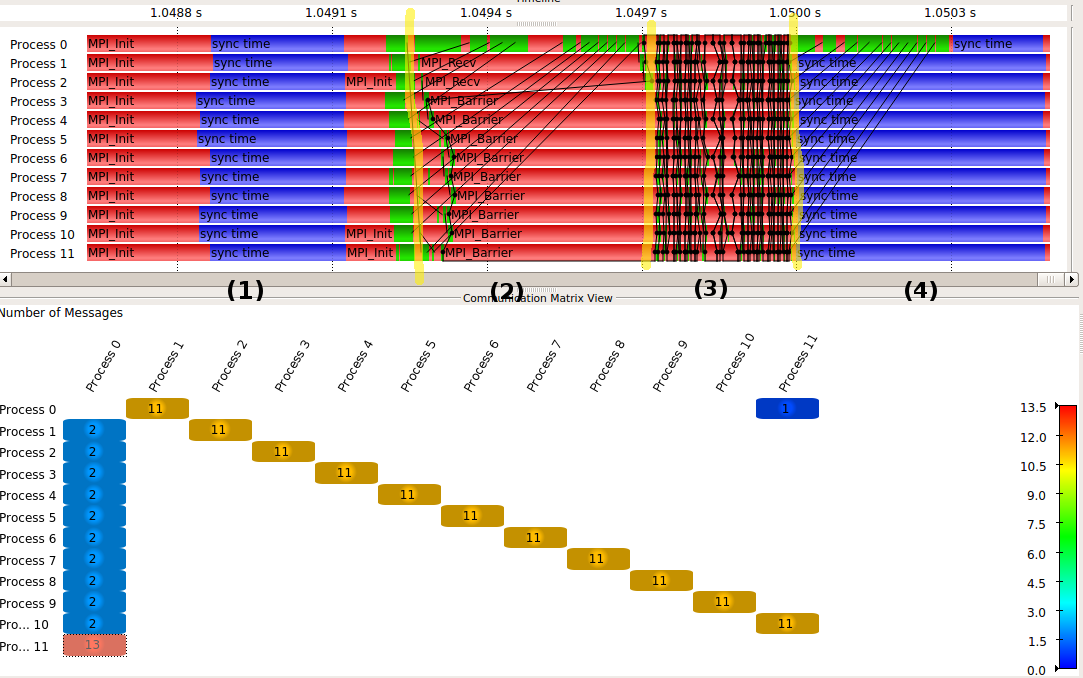
\includegraphics[width=1\textwidth]{./vampir/phasen_numnachrichten.png}

Im oberen Bereich ist die Timeline zu sehen, jeder waagerechte Balken stellt einen Prozess dar.
Eine schwarzen Linie zwischen zwei Prozessen steht für einen Nachrichtenaustausch.
In unserem Fall sind die MPI Routinen rot dargestellt, Funktionen des eigentlichen Programms sind grün.
\begin{enumerate}
 \item[Abschnitt (1):]~\\
Dieser Abschnitt gehört noch zu Initalisierung
\item[Abschnitt (2):]~\\
Hier berechnet jeder Prozess die Länge seines Teilarrays und füllt dieses mit zufälligen Zahlen.
Dann werden diese für die Ausgabe ``Before'' an den Masterprozess gesendet.
\item[Abschnitt (3):]~\\
Der dritte Abschnitt zeigt die Iterationen.
\item[Abschnitt (4):]~\\
Im vierten Abschnitt sendet jeder Prozess sein aktuelles Teilarray zum Masterprozess, damit dieses es ausgeben kann.
Danach folgt die Beendung.
\end{enumerate}

Im unteren Bereich des Bildes ist die ``Communication Matrix View'' zu sehen, hier wird die Anzahl der Kommunikationen zwischen den Prozessen gezeigt.
Man kann hier schön sehen, dass jeder Prozess außer dem Masterprozess 2 mal an den Masterprozess sendet, nämlich jeweils für die Ausgaben.
Der Masterprozess sendet einmal an den letzten Prozess um ihm das erste Element im Array mitzuteilen.
Außerdem kommuniziert jeder Prozess 11 mal mit seinem Nachfolger.
\newpage
Vergrößert man nun den Auschnitt (3), der die Iteration zeigt noch weiter, kann man den Austausch der Nachrichten sehen:\\
~\\
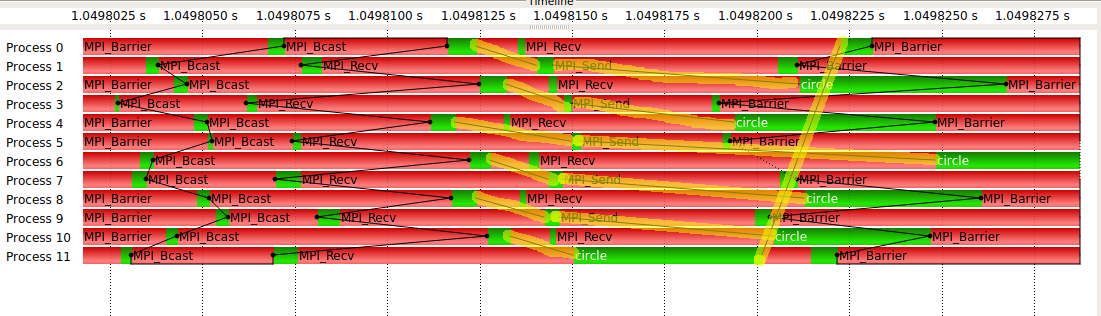
\includegraphics[width=1\textwidth]{./vampir/Nachrichtenaustausch.png}
Hier senden zuerst die Prozesse mit gerade Zahl ihre Werte an den nächsten Prozess, danach die Prozesse mit ungerader Zahl.
Die Prozesse kommunizieren also wie erwartet.

\end{document}
